% Created 2023-01-17 Ter 15:07
% Intended LaTeX compiler: pdflatex
\documentclass[article,12pt,openany,oneside,a4paper,chapter=TITLE,hyphen,english,brazil,chapter=TITLE,sumario=tradicional]{abntex2}
                  \usepackage{nopageno}
\usepackage{pdfpages}
\usepackage{times}
\usepackage[utf8]{inputenc}
\usepackage[T1]{fontenc}
\usepackage{color}
\usepackage{microtype}
\usepackage{titlesec}
\usepackage[brazilian, hyperpageref]{backref}
\usepackage{hyperref}
\usepackage[alf,abnt-emphasize=bf,abnt-doi=link]{abntex2cite}
\usepackage{indentfirst}
\usepackage{listings}
\usepackage{graphicx}
\usepackage{lipsum}
\usepackage{amssymb}
\usepackage{amsmath}
\lstset{basicstyle=\ttfamily\small,breaklines=true}
\titleformat{\section}{\normalfont\normalsize\bfseries\uppercase}{}{0pt}{}
\titleformat{\subsection}{\normalfont\normalsize\bfseries}{}{0pt}{\space}
\titleformat{\subsubsection}{\normalfont\normalsize\bfseries}{}{0pt}{\space}
\titleformat{\paragraph}{\normalfont\normalsize\itshape}{}{0pt}{\theparagraph\space}
\setlength{\parindent}{1.5cm}
\setlrmarginsandblock{3cm}{2cm}{*}
\setulmarginsandblock{2.5cm}{2.5cm}{*}
\checkandfixthelayout
\renewcommand{\backrefpagesname}{Citado na(s) página(s):~}
\renewcommand{\backref}{}
\renewcommand*{\backrefalt}[4]{}
\makeindex
\titulo{Partitura para Oficina de Música de Curitiba 2023}
\author{Davi Raubach}
\local{Pelotas}
\author{Davi Raubach}
\date{}
\title{omcwb}
\hypersetup{
 pdfauthor={Davi Raubach},
 pdftitle={omcwb},
 pdfkeywords={},
 pdfsubject={},
 pdfcreator={Emacs 29.0.50 (Org mode 9.5.4)}, 
 pdflang={Bt-Br}}
\begin{document}

\OnehalfSpacing

\pretextual

\imprimircapa
\newpage

\begin{dedicatoria}
\vspace*{\fill}
Esta é uma dedicatória.

\vspace*{\fill}
\end{dedicatoria}
\newpage

\begin{epigrafe}
\vspace*{\fill}
Nunca nos curamos de ter sonhado ao pé de uma água dormente\ldots{}
Gaston Bachelard
\vspace*{\fill}
\end{epigrafe}
\newpage



\textual


\section*{Prefácio}
\label{sec:orge44c1e8}
Nesta composição, a leitura de um texto verbal ocupa uma posição de geração de material musical e de organizador relativo da temporalidade. Em boa parte da peça, o passar do tempo é articulado pela leitura do texto.

O poema abaixo cumpre essa função na peça foi escrito para essa ocasião.

\begin{center}


Palavra atirada contra a água\\
Salta, salta, voa\\
Pousa sobre as nuvens\\
Mergulha cada vez mais fundo\\
Cada vez mais alto\\
Seduz a língua e escoa\\
Escoa, salta, voa\\
Cada vez mais sonhada
\end{center}


\section*{Notas de Performance}
\label{sec:org5e5cd7d}

\textbf{Duração} c. 4 min

\subsection*{Notação rítmica}
\label{sec:org523ab70}

\subsubsection*{Tempo estrito}
\label{sec:orgcc2e305}

Notado tradicionalmente

\subsubsection*{Tempo de leitura}
\label{sec:org1da9c46}

Gestos instrumentais estão associados às sílabas do texto. O/A intérprete deve executar a música levando em conta sua associação com o texto. A leitura do texto determina quando tocar. 

\begin{itemize}
\item Leitura mental
\label{sec:org1d8b387}

Texto em tachado indica que não se deve ler em voz alta, apenas mentalmente (esse é o caso em toda peça, por enquanto).

\begin{itemize}
\item Cabeça de nota como de semínima representa a leitura de uma sílaba para cada nota (notas mais curtas).
\item Cabeça de nota como de mínimas representam notas que se estendem por várias sílabas (notas mais longas):
\end{itemize}

\begin{center}
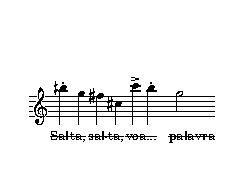
\includegraphics[width=7cm]{exemplo_tempo_fala.pdf}
\end{center}

Além disso, um sinal de respiração indica os limites de som e pausa.

\item Modos de fala
\label{sec:org1b63f6a}

O modo da leitura mental também está indicado e pode ser \emph{poético}, como a leitura de um poema por Pablo Neruda, ou \emph{dramático}, como uma fala de protesto. A primeira é uma leitura mais lenta, enquanto a segunda é mais rápida.

\item Conflitos entre leitura musical e textual
\label{sec:orgd691522}

Em geral, o ritmo instrumental deve se submeter ao ritmo da leitura. Entretanto, também deve-se levar em consideração que alguns gestos precisam de tempo hábil para a execução e nestes casos não há problema em suspender o tempo da leitura.

\item Sincronia
\label{sec:orgb247972}

Por causa da diferença da leitura de cada intérprete, muitos momentos não exigem sincronia, com exceção de início de seções e momentos específicoos indicados com  \textbf{barras de compasso pontilhadas, que representam momentos de retomada da sincronia}.
\end{itemize}

\subsection*{Multifônicos Sax}
\label{sec:orga2fb72c}

Anotei na partitura o multifônico de acordo com os nomes abaixo. Escrevi todas as notas, mas a ideia é conferir as possibilidades de cada multifônico e anotar as notas mais especificamente. 

M1:

\begin{center}
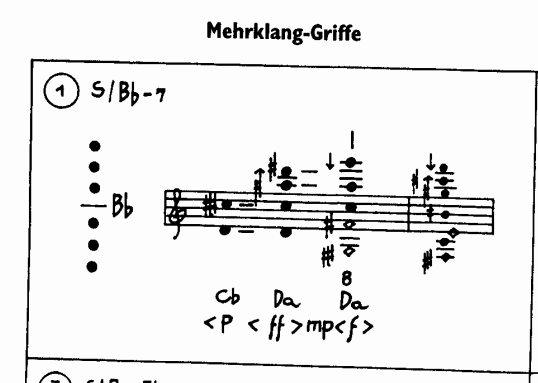
\includegraphics[width=8cm]{images/multi1.png}
\end{center}

M2:

\begin{center}
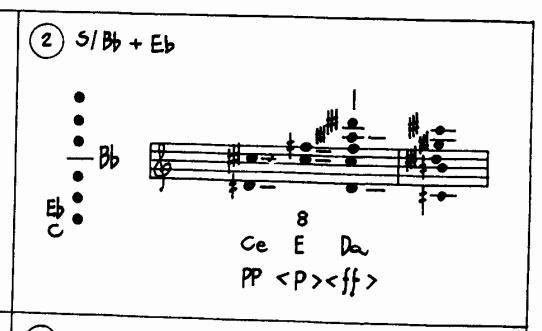
\includegraphics[width=8cm]{images/multi2.png}
\end{center}


M7:

\begin{center}
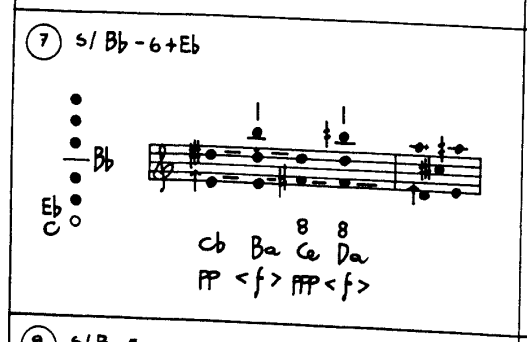
\includegraphics[width=8cm]{images/multi7.png}
\end{center}

M15:

\begin{center}
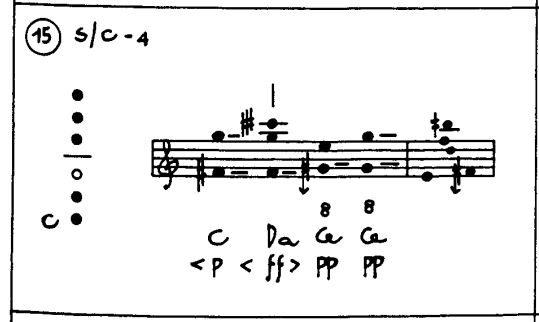
\includegraphics[width=8cm]{images/multi15.png}
\end{center}

M31:

M77:

\begin{center}
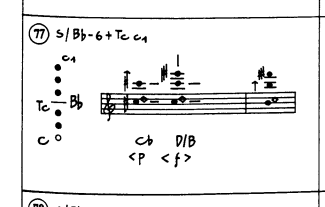
\includegraphics[width=8cm]{images/multi77.png}
\end{center}

Retirados de WEISS, Marcus; NETTI, Giorgio. The techniques of saxophone playing. Bärenreiter, 2010

\section*{Processo}
\label{sec:orge3aad50}
Gostaria de mencionar que terminei essa primeira versão com muita pressa e posso estar deixando passar alguma coisa (inclusive simples). Com a pressa, também optei por coisas que mudaria se for possível. Por exemplo:
\begin{itemize}
\item mudar o material do cello na primeira seção
\item melhorar o uso das técnicas da flauta para ter uma gradação entre whitle tones e slap tongue
\item pensar nas técnicas do cello na segunda seção
\item definir melhor as notas alvo dos multifônicos do sax
\item ser mais preciso nas dinâmicas
\end{itemize}

Gostaria ainda de acrescentar uma transição entre as duas seções, algo com cerca de 15 segundos e também uma coda com duração semelhante.

\section*{Contágios}
\label{sec:org85df8b4}
\begin{itemize}
\item Utilização dos multifônicos do saxophone como gerador de alturas (Charles Neimog)
\item Modulação de frequências para derivação de alturas (Bruno Gageiro)
\end{itemize}

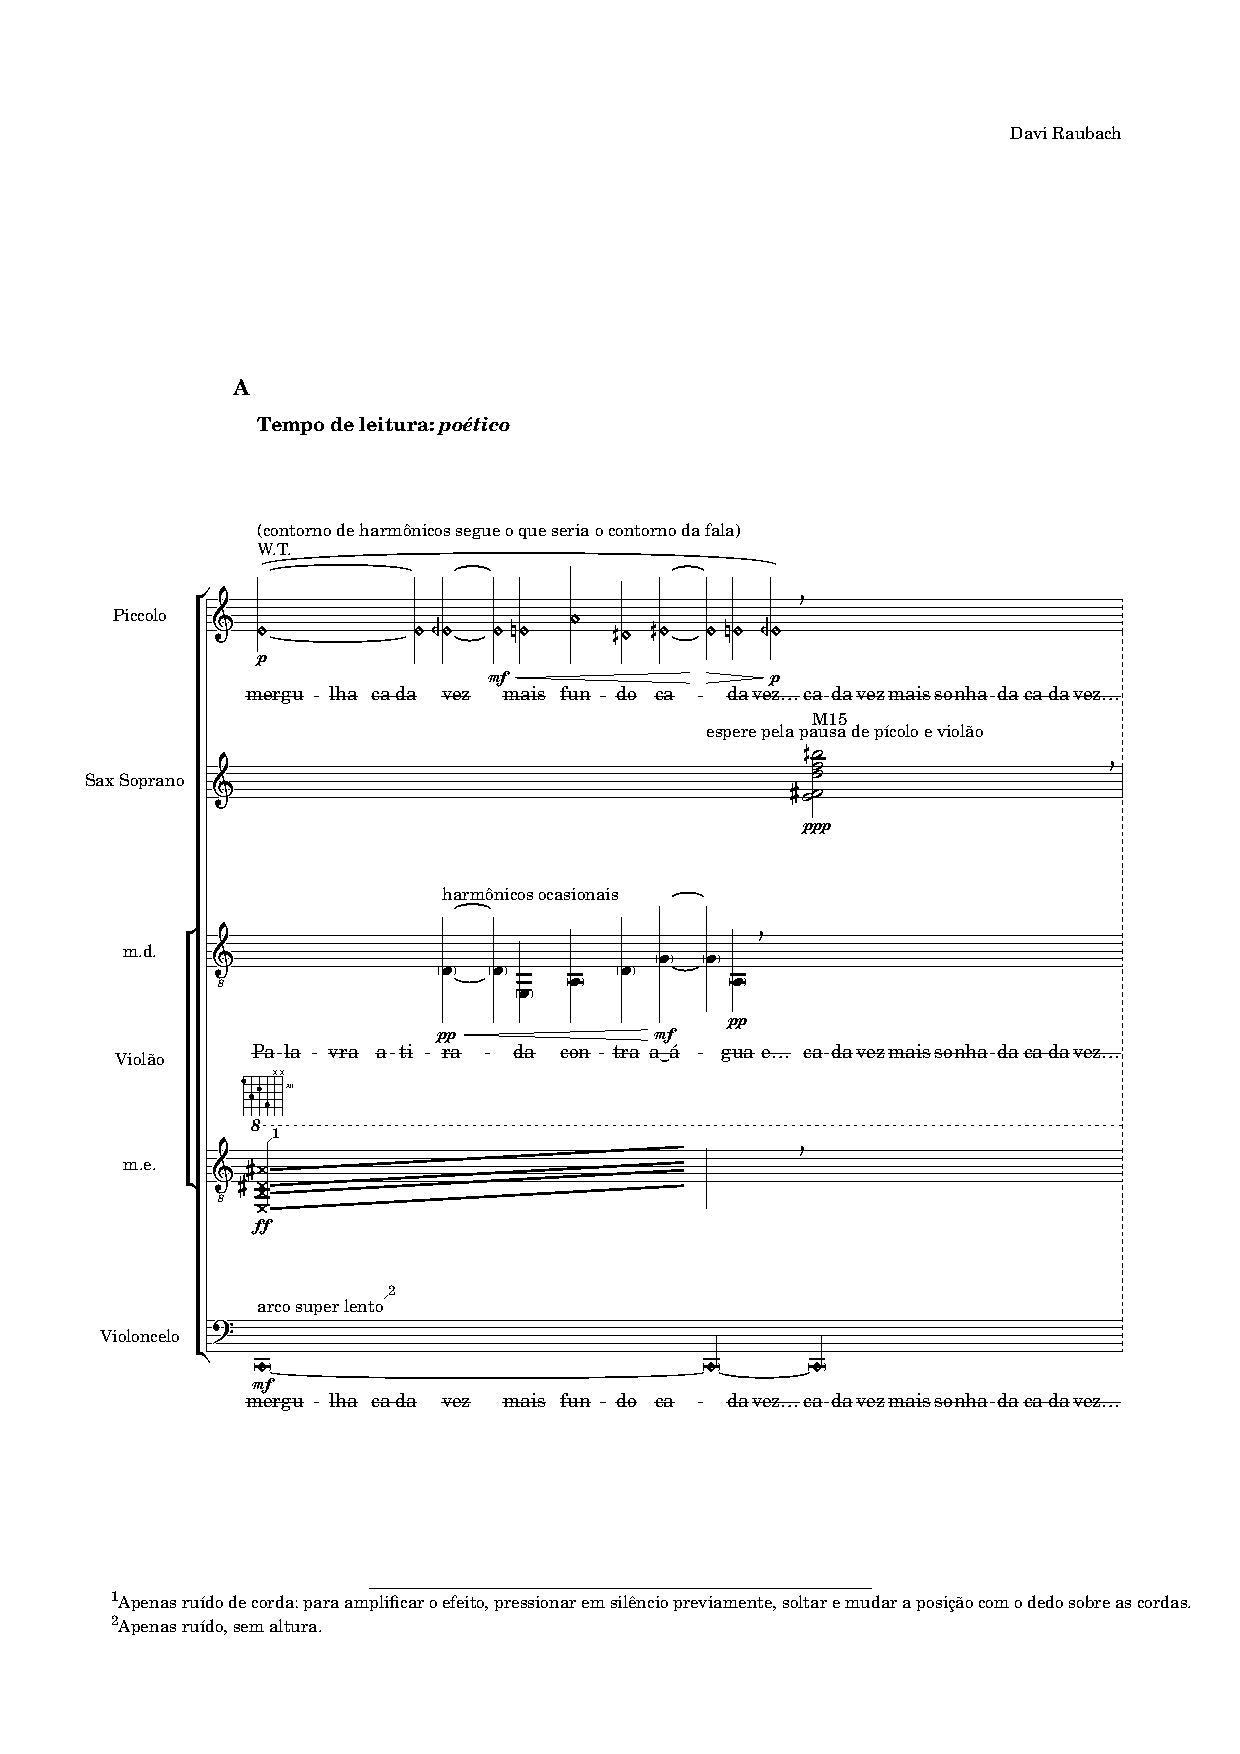
\includepdf[pages=-,pagecommand={}]{omcwb_score.pdf}
\end{document}